\documentclass[12pt,a4paper]{report}
\usepackage{amssymb,amsmath}
\usepackage[utf8]{inputenc}
\usepackage[spanish]{babel}
\selectlanguage{spanish}
\usepackage{graphicx}
\usepackage{pgfplots}
\usepackage{tikz}
\usepackage{enumerate}
\usepackage{listings}
\usepackage[T1]{fontenc}
\usepackage{mathrsfs} 
\lstset{language=Matlab, breaklines=true, basicstyle=\footnotesize}
\lstset{numbers=left, numberstyle=\tiny, stepnumber=1, numbersep=-8pt}
\usepackage{cite} % para contraer referencias
%%formato de leonel 
\setlength{\voffset}{0pt}

\setlength{\topmargin}{-32pt}
\setlength{\headheight}{20pt}
\setlength{\headsep}{19pt}
\setlength{\topskip}{0pt}

\setlength{\oddsidemargin}{0pt}
\setlength{\evensidemargin}{0pt}
\setlength{\marginparwidth}{0.75in}
\setlength{\marginparsep}{0.1in}

\setlength{\abovecaptionskip}{3pt}
\setlength{\footskip}{30pt}

\setlength{\textwidth}{\paperwidth}
\addtolength{\textwidth}{-2in}
\setlength{\textheight}{\paperheight}
\addtolength{\textheight}{-1.75in}

\setlength{\parindent}{1em}
\setlength{\parskip}{0.3em}
%%leonel

\begin{document}
%%portada
\begin{titlepage}
%%portada
		\begin{center}
			\vspace*{-1in}
			\begin{figure}[htb]
			\centering
					
\includegraphics[scale=0.2]{logo_original}
			\end{figure}
			
			TECNOLÓGICO NACIONAL DE MÉXICO\\
			\vspace*{0.15in}
			INSTITUTO TECNOLÓGICO DE MORELIA \\
			\vspace*{0.3in}
			\begin{large}
				DEPARTAMENTO DE INGENIERÍA ELECTRÓNICA\\
			\end{large}
			\vspace*{0.2in}
			\begin{large}
				CONTROL 1\\
			\end{large}
		\vspace*{0.3in}
			\begin{Large}
				\textbf{Práctica 1\\
				sistema hidraulico} \\
			\end{Large}
			\vspace*{0.3in}
			\begin{large}
			Profesor: Gerardo Marx Chávez Campos\\
			\end{large}
			\vspace*{0.2in}
		\begin{large}
			Alumnos : \\
			Carlos Ivan Ramírez Arguello\\
			Edrei Martinez Lopez \\
		\end{large}
			\vspace*{0.3in}
			\rule{80mm}{0.1mm}\\
			\vspace*{0.1in}
			\begin{large}
				MORELIA, MICHOACÁN \\
				Fecha de Entrega:\\
				27/octubre/2017 \\
			\end{large}
		\end{center}
	\end{titlepage}
%%portada
%%reporte
\tableofcontents
\chapter{Introducción}
Trabajar en el dominio de la frecuencia, no solamente es útil para la resolución matemática de
ecuaciones sino que se presta especialmente para ser utilizado con el concepto de
función de transferencia. En general un proceso recibe una entrada $u(t)$ y genera una
salida $y(t)$. Si llevamos estas señales al dominio de LAPLACE tendremos una entrada
$U(s)$ que genera una salida $Y(s)$. La función que relaciona salida con entrada se
denomina función de transferencia $g(s)$.\\
\begin{figure}[h!]
  \centering
    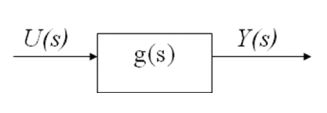
\includegraphics[width=4.0in]{funciontransferencia}
  \caption{Función de Transferencia}
\end{figure}
De modo que :$Y(s) = g(s)*U(s).$
Sistemas de primer orden
Se denominan sistemas de primer orden a aquellos en los que en la ecuación general
aparece solamente la derivada primera del lado izquierdo (el de la variable de estado). O
sea que se reducen al formato siguiente:
\begin{equation}
\tau\frac{dy}{dt}+y= k*u
\end{equation}
donde $k$ se denomina ganancia del proceso y $\tau$ es la constante de tiempo del sistema.
En general encontraremos que la ecuación está escrita en función de las variables
“desviación” respecto al valor de estado estacionario. Por lo tanto en general $y(0) = 0 ,
u(0) = 0$ . Tomando transformadas de LAPLACE.\ref{ft}
\begin{equation*}
\tau [s Y(s)-y(0)]+Y(s)=kU(s)
\end{equation*}
\begin{equation*}
\tau s Y(s)+ \tau Y(s)=kU(s)
\end{equation*}
\begin{equation*}
( \tau s+1)Y(s)=kU(s)
\end{equation*}
\begin{equation*}
Y(s)=\frac{k}{\tau s+1}U(s)
\end{equation*}
\begin{equation*}
Y(s)=g(s)U(s)
\end{equation*}
\begin{equation*}
g(s)=\frac{k}{\tau s+1}
\end{equation*}
\chapter{Metodología}
Primero considerando la ecuación general de la función de transferencia:
\begin{equation}
H(s)=\frac{bs+c}{s+a}
\end{equation}
para obtener la respuesta de paso se tiene que multiplicar $H(s)$ por la función escalón:
\begin{equation}
Y(s)=\frac{1}{s}\frac{bs+c}{s+a}
\end{equation}
\section{Fracciones Parciales}
seguido de esta multiplicación se aplican fracciones parciales para obtener los valores de A y B de estas mismas para poder hacer una sustitución en la transformada inversa de LAPLACE:
\begin{equation*}
Y(s)=\frac{bs+c}{s(s+a)}
\end{equation*}
\begin{equation*}
\frac{bs+c}{s(s+a)}=\frac{A}{s}+\frac{B}{s+a}
\end{equation*}
para $s=0$:
\begin{equation*}
bs+c=A(s+a)+Bs
\end{equation*}
\begin{equation*}
0+c=A(0+a)+0
\end{equation*}
\begin{equation*}
A=\frac{c}{a}
\end{equation*}
para $s=-a$
\begin{equation*}
b(-a)+c=A(-a+a)+B(-a)
\end{equation*}
\begin{equation*}
b(-a)+c=A0+B(-a)
\end{equation*}
\begin{equation*}
B=\frac{(-a)b+c}{-a}
\end{equation*}
\section{Sustitución en LAPLACE INVERSA}
ya de haber obtenido los coeficientes de A y B se aplica LAPLACE inversa:
\begin{equation}
\mathscr{L^{-1}}\{f(t)\} = \mathscr{L^{-1}}\{\frac{c}{a}+\frac{(-a)b+c}{-a}\} 
\end{equation}
\begin{equation}
\mathscr{L^{-1}}\{f(t)\} = \frac{c}{a}+\frac{(-a)b+c}{-a}e^{-at} 
\end{equation}
\chapter{Resultados}
La función que fue proporcionada en la practica es la siguiente la cual nos da una respuesta exponencial en la parte donde se desborda nuestro tinaco por que entra mas cantidad de agua de la que sale por lo que es un punto critico en nuestro sistema ,este mismo tiene que tener una equilibrio para tener un sistema optimizado.\\

código en Scilab del profesor:
\begin{lstlisting}[frame=single]
s =%s
poly (0 , 's')
K =1;
Tau =1;
simpleSys=syslin('c' , K/(1+Tau*s)) //funcio de transferencia
t=0:0.01:1;
y=csim('step', t, simpleSys)//funcion escalon step
plot(t,y)
xlabel('respuesta en el timepo')
ylabel('nivel del agua')

\end{lstlisting}
En la siguiente figura se muestra la gráfica arrojada por el código anterior:\\
\begin{figure}[h!]
  \centering
    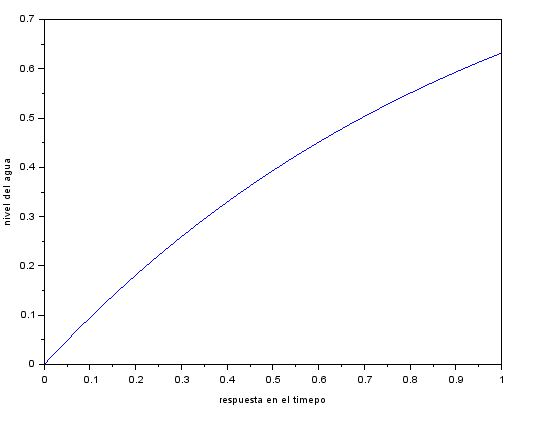
\includegraphics[width=4.0in]{IMAGENPROFE}
  \caption{Respuesta de salid cuando es mayor la entrada que la salida de agua}
\end{figure}
En el siguiente código y gráfica es una representación real del sistema en distintos puntos críticos los cuales los orientan para poder obtener valores de nuestros dispositivos  para el buen funcionamiento de este ,primero se muestra una gráfica cuando ingresa mayor cantidad de agua al sistema pero sale menor cantidad de agua ,en la segunda es un sistema estable por lo cual la respuesta en una linea por que hay un equilibrio entre entrada y salida ,en la ultima y tercera gráfica se muestra cuando la llave en la salida esta abierta y hay poca agua ingresando al contenedor de agua.
código en Matlab :
\begin{lstlisting}[frame=single]
  clear all
  clc
  c=3;
  a=1;
  b=0;
  t=0:0.01:10;
  y=((c/a)-((-a*b+c)/a)*exp(- a*t));
  subplot(3,1,1)
  plot(t,y);
  xlabel('respuesta en el timepo')
  ylabel('nivel del agua ')
  % %%%%%%% entrada igual que la salida
  clear all
  cc=1;
  aa=1;
  bb=1;
  t2=0:0.01:10;
  y2=((cc/aa)+((aa*bb-cc)/aa)*exp(-1*aa*t2));
  subplot(3,1,2)
  plot(t2,y2);
  xlabel('respuesta en el timepo')
  ylabel('nivel del agua ')
  %%%%%%%%
  clear all
  ccc=1;
  aaa=1;
  bbb=5;
  t3=0:0.01:10;
  y3=((ccc/aaa)-((-aaa*bbb+ccc)/aaa)*exp(-1*aaa*t3));
  subplot(3,1,3)
  plot(t3,y3);
  xlabel('respuesta en el timepo')
  ylabel('nivel del agua ')

\end{lstlisting}
En la siguiente figura se observa las graficas del código implementado en laboratorio en Matlab:
\begin{figure}[h!]
  \centering
    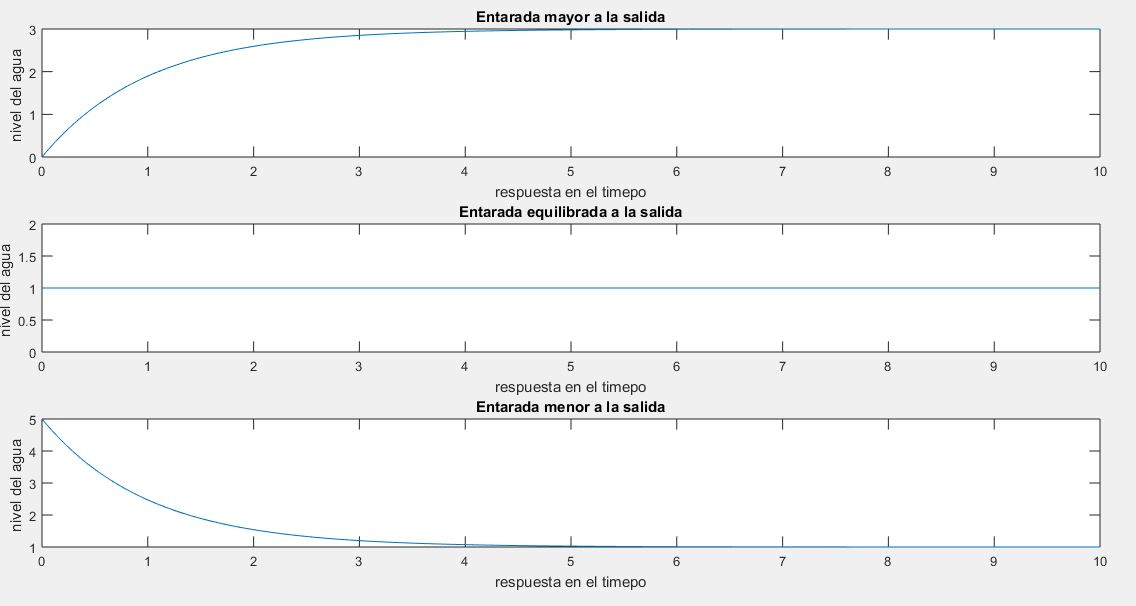
\includegraphics[width=6.0in]{codmio}
  \caption{Respuesta de entrada contra salida en los 3 casos.}
\end{figure}
\newpage
\chapter{conclusiones}
Carlos Ivan Ramirez Arguello\\

La práctica,consistió en encontrar la función de transferencia ,así poder encontrar una relación de entrada con la salida por lo que al obtener la función de transferencia queremos nuestra función que describe el funcionamiento de nuestro sistema,algo muy útil de la práctica es esto por lo cual podemos hacer una representación o un modelo matemático el cual nos puede interpretar cual es el dispositivo o punto donde afecta el sistema y lo puede llevar a un punto  critico de funcionamiento.Las fracciones parciales fundamentales para la resolución de estos problemas por lo que se aplica para obtener la función descriptiva y así aplicar LAPLACE inversa para ver la respuesta en función del tiempo. \\

Edrei Martinez Lopez\\

Al nosotros estar trabajando con LAPLACE no solamente se nos es útil para la resolución matemática de ecuaciones sino que también se utiliza especialmente para el concepto de función de transferencia. La función que relaciona salida con entrada se denomina función de transferencia g(s). Al sacar nuestra respuesta de la función, considerando la función de transferencia genérica, la respuesta al escalón se obtiene al tomar la transformada inversa donde k y tao son la ganancia del sistema y la constante de tiempo así obteniendo nuestra respuesta del sistema, en dicho ejercicio del sistema hidráulico sacando su respuesta obtuvimos nuestras gráficas.

\chapter{Referencias}
$http://grupovirtus.org/moodle/pluginfile.php/3799/mod_resource/content\\/1/SEMANA_2/Sistemas_dinamicos_de_primer_orden.pdf$\label{ft} 


\end{document}
